\documentclass{sigchi}

% Use this command to override the default ACM copyright statement (e.g. for preprints). 
% Consult the conference website for the camera-ready copyright statement.


%% EXAMPLE BEGIN -- HOW TO OVERRIDE THE DEFAULT COPYRIGHT STRIP -- (July 22, 2013 - Paul Baumann)
% \toappear{Permission to make digital or hard copies of all or part of this work for personal or classroom use is 	granted without fee provided that copies are not made or distributed for profit or commercial advantage and that copies bear this notice and the full citation on the first page. Copyrights for components of this work owned by others than ACM must be honored. Abstracting with credit is permitted. To copy otherwise, or republish, to post on servers or to redistribute to lists, requires prior specific permission and/or a fee. Request permissions from permissions@acm.org. \\
% {\emph{CHI'14}}, April 26--May 1, 2014, Toronto, Canada. \\
% Copyright \copyright~2014 ACM ISBN/14/04...\$15.00. \\
% DOI string from ACM form confirmation}
%% EXAMPLE END -- HOW TO OVERRIDE THE DEFAULT COPYRIGHT STRIP -- (July 22, 2013 - Paul Baumann)


% Arabic page numbers for submission. 
% Remove this line to eliminate page numbers for the camera ready copy
% \pagenumbering{arabic}


% Load basic packages
\usepackage{balance}  % to better equalize the last page
\usepackage{graphics} % for EPS, load graphicx instead
\usepackage{times}    % comment if you want LaTeX's default font
\usepackage{url}      % llt: nicely formatted URLs

% llt: Define a global style for URLs, rather that the default one
\makeatletter
\def\url@leostyle{%
  \@ifundefined{selectfont}{\def\UrlFont{\sf}}{\def\UrlFont{\small\bf\ttfamily}}}
\makeatother
\urlstyle{leo}


% To make various LaTeX processors do the right thing with page size.
\def\pprw{8.5in}
\def\pprh{11in}
\special{papersize=\pprw,\pprh}
\setlength{\paperwidth}{\pprw}
\setlength{\paperheight}{\pprh}
\setlength{\pdfpagewidth}{\pprw}
\setlength{\pdfpageheight}{\pprh}

% Make sure hyperref comes last of your loaded packages, 
% to give it a fighting chance of not being over-written, 
% since its job is to redefine many LaTeX commands.
\usepackage[pdftex]{hyperref}
\hypersetup{
pdftitle={SIGCHI Conference Proceedings Format},
pdfauthor={LaTeX},
pdfkeywords={HCI, Cooperative, Spaceship, Game},
bookmarksnumbered,
pdfstartview={FitH},
colorlinks,
citecolor=black,
filecolor=black,
linkcolor=black,
urlcolor=black,
breaklinks=true,
}

% create a shortcut to typeset table headings
\newcommand\tabhead[1]{\small\textbf{#1}}


% End of preamble. Here it comes the document.
\begin{document}

\title{CSG: A communicative Game for Interactive Floors}

\numberofauthors{1}
\author{
  \alignauthor Daniel Birnstiel, Patrick Kuhn, Fabian Paul, Lennard Wolf\\
      \medskip
    \affaddr{Hasso Plattner Institute}\\
    \affaddr{Prof.-Dr.-Helmert-Str. 2-3}\\
    \affaddr{14482 Potsdam, Germany}\\
    \email{$ \{ $ daniel.birnstiel, patrick.kuhn, fabian.paul, lennard.wolf $ \} $@student.hpi.de }\\
}

\maketitle

\begin{abstract}

After looking upon the possibilities of interactive floors and taking into account the immense demand for, and market of video games today, we developed \textit{CSG}, or \textit {Cooperative Spaceship Game}. It is meant as a prototype for communicative, interactive floor based games and demonstrates, how playing games at home can once again involve movement of the whole body - and not just the thumbs.

The players' goal is the joint reaching of levels by performing tasks that are created at random. These tasks may involve actions which the player, who was given said task, may not be able to carry out. Thus he/she has to tell their partner(s) to execute it.

\end{abstract}

\keywords{
	Cooperative Spaceship Game; Communication; Interactive Floors; Body Movement
}


\section{Introduction}

With the advent of the \textit {Internet of Things} and thus the rising digital Interaction with everything around us, floors will soon become intelligent entities just like our phones are today. 

But next to all the productive things we can now do with our devices, we also want to integrate them into our leisure time. Just like touch screens revolutionized the way we play games, interactive floors will again push the boundaries of the way we think about enjoying ourselves through games.

To understand what players want from a game, we interviewed a professional Game Designer, a Game Design Lecturer as well as a few gamers - both casual and somewhat professional. We learned that nowadays players have a lower attention span and thus want to understand the game right away. This is why we started out contemplating different mini games and at some point even considered a mini game collection. But what we saw as the main advantage of an interactive floor based game was the fact that the player might not be alone, but rather be in the same room with others and cooperate. 

This is why we chose to concentrate on three main goals for our project: \textbf{Communication}, \textbf{Cooperation} and \textbf{Discoverability}.



\begin{figure}[!h]
\centering
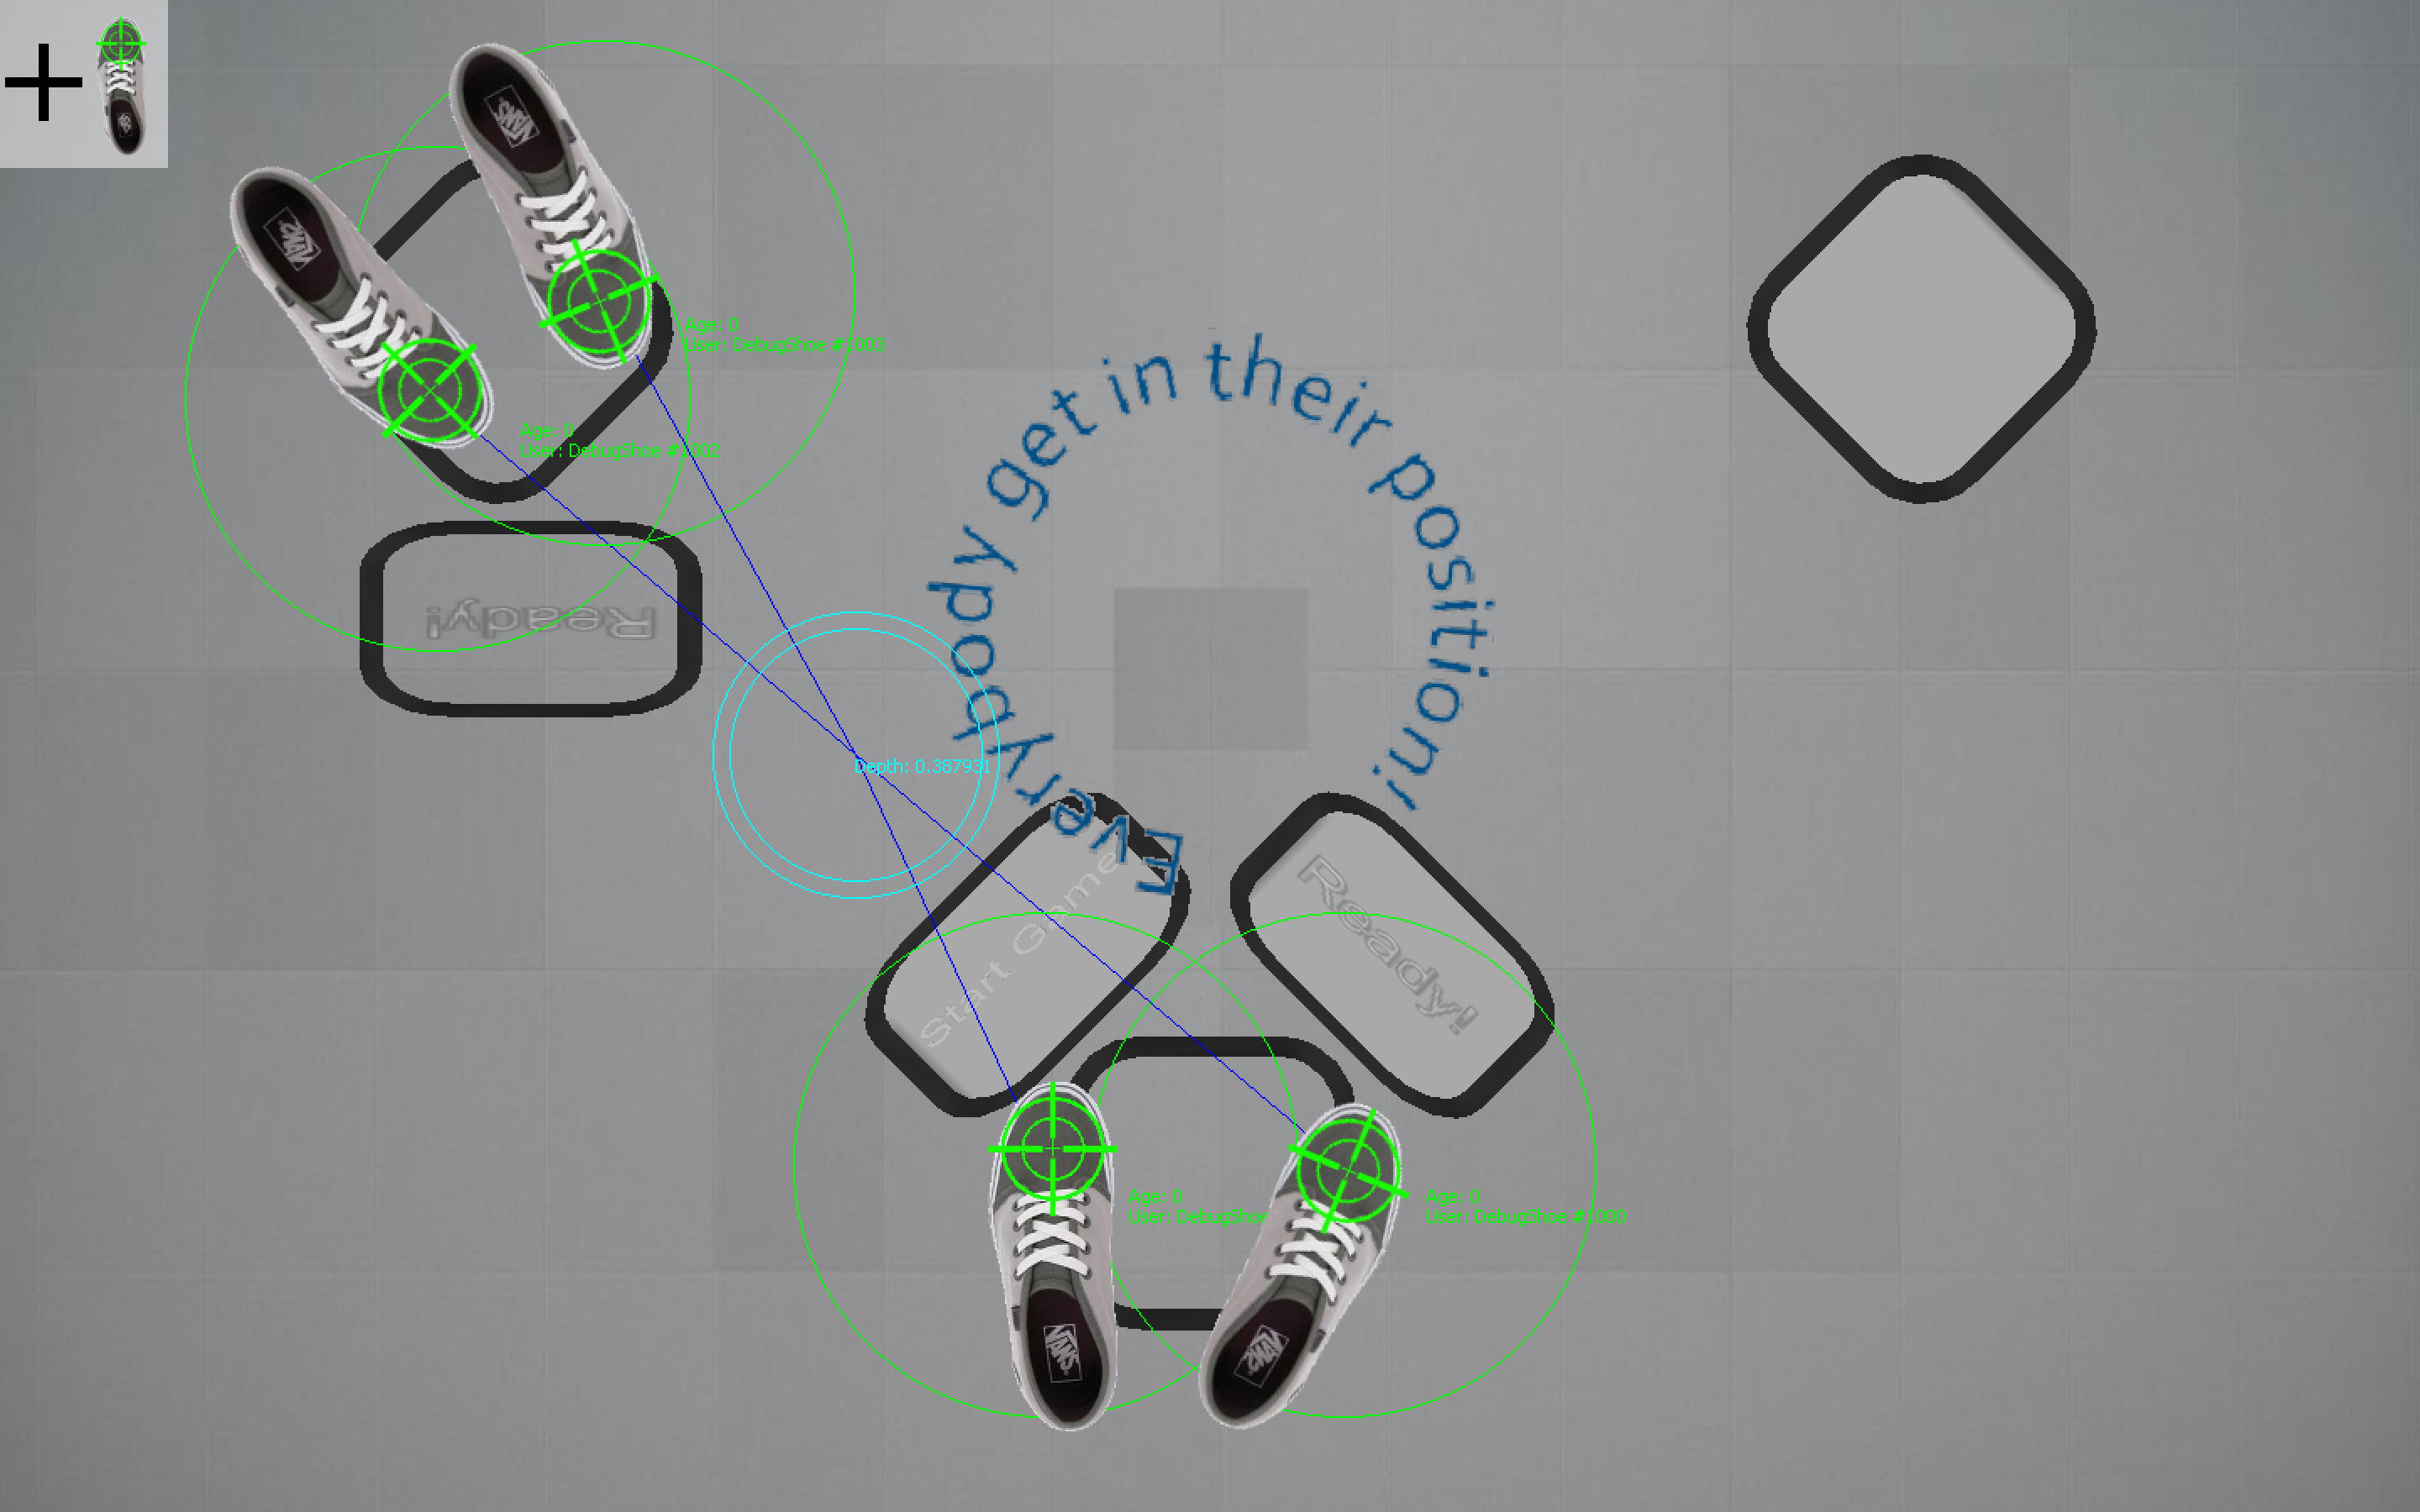
\includegraphics[width=0.9\columnwidth]{Figure1}
\caption{Here you can see the beaming area.}
\label{fig:figure1}
\end{figure}

\section{The Concept of the game}

Hier wird das spielprinzip erklärt

\section{Walkthrough}

In our scenario two users X and Y want to play the game. As shown in figure? both users enter the floor and they will get in \textit{the Beaming Area}.

\subsection{The Beaming Area}

1.1 - Users walk to their platforms. 1.2 - Appeared ready buttons will change the ? to a ! after stepping on it.
1.3 - User A (first entered the platform) get a start button and tap on it


\subsection{The Gaming Area}

2.1 - User X and Y follow the arrows to their instruction panels
2.2 - Instruction will be given to the both Users.
2.3 - The two timer starts ticking and both try to fulfill their task by communicating and find their issues. 
2.4 User X have to change the slider state <....> .
2.5 User Y have to change the spinner <...> on 6.
2.4 - After succeeding their tasks new will be generated. The timer resets once every task is successfully done and start with decremented duration.
2.5 Game finish if anyone tap on the elevator button.



\section{Design}


\subsection{Design Concept 1}

Cooperation as game principle
Our first idea was to create an application, which consists of various minigames that can be successively played against each other. The problem with this approach was, as Willi Scheibel pointed out in our contextual inquiry, that it doesn't allow users to interact with each other. 

So in our new design we integrate cooperation as game principle by adding tasks which have to be performed by both users. Moreover we use the spatial distribution of our tasks to encourage interaction between the players, rather than having them perform only their own tasks. 
 
\subsection{Design Concept 2}

Standing in defined area as login mechanism 
Initially we thought about having the user register to the system with an on-floor keyboard and then log in every time he enters the floor. We encountered in paper prototyping that it is really tedious for the user to type in his name, since tapping on small buttons requires precision and having the buttons spread makes them hard to use because it would be nessecary to walk over them to get to the destination. 

We decided to use an predefined area in which the user has to stand to start the game. The paper prototyping and the heuristic evaluation showed that this was easily recognizable. 
***Here maybe be a picture of the beaming area*** 


\subsection{Design Concept 3}

Avoiding roles as game mechanic
Originally we came up with the idea of having different roles who are able to carry out certain tasks. For example role of the captain was assigned to the first person entering a beaming platform and was able to start the game. In our paper prototyping, most of the testers asked about the meaning of the roles. Explaining the concept at this time in the game would require adding a tutorial and make the game harder to discover. 

In our final design we replaced the concept of roles by making tasks more specific.   

\subsection{Design Concept 4}

Warum ist unser Design immer noch das beste für den job?



\subsection{References and Citations}

Use a numbered list of references at the end of the article, ordered
alphabetically by first author, and referenced by numbers in brackets
\cite{ethics,
  Klemmer:2002:WSC:503376.503378,
  Mather:2000:MUT,
  Zellweger:2001:FAO:504216.504224}. For
papers from conference proceedings, include the title of the paper and
an abbreviated name of the conference (e.g., for Interact 2003
proceedings, use \textit{Proc. Interact 2003}). Do not include the
location of the conference or the exact date; do include the page
numbers if available. See the examples of citations at the end of this
document. Within this template file, use the \texttt{References} style
for the text of your citation.

Your references should be published materials accessible to the
public.  Internal technical reports may be cited only if they are
easily accessible (i.e., you provide the address for obtaining the
report within your citation) and may be obtained by any reader for a
nominal fee.  Proprietary information may not be cited. Private
communications should be acknowledged in the main text, not referenced
(e.g., ``[Robertson, personal communication]'').

\begin{table}
  \centering
  \begin{tabular}{|c|c|c|}
    \hline
    \tabhead{Objects} &
    \multicolumn{1}{|p{0.3\columnwidth}|}{\centering\tabhead{Caption --- pre-2002}} &
    \multicolumn{1}{|p{0.4\columnwidth}|}{\centering\tabhead{Caption --- 2003 and afterwards}} \\
    \hline
    Tables & Above & Below \\
    \hline
    Figures & Below & Below \\
    \hline
  \end{tabular}
  \caption{Table captions should be placed below the table.}
  \label{tab:table1}
\end{table}

\section{Sections}

The heading of a section should be in Helvetica 9-point bold, all in
capitals. Use Arial if Helvetica is not available. Sections should
not be numbered.

\subsection{Subsections}

Headings of subsections should be in Helvetica 9-point bold with
initial letters capitalized.  For
sub-sections and sub-subsections, a word like \emph{the} or \emph{of}
is not capitalized unless it is the first word of the heading.)

\subsubsection{Sub-subsections}

Headings for sub-subsections should be in Helvetica 9-point italic
with initial letters capitalized.  Standard {\textbackslash}section,
{\textbackslash}subsection, and {\textbackslash}subsubsection commands
will work fine.

\section{Figures/Captions}

Place figures and tables at the top or bottom of the appropriate
column or columns, on the same page as the relevant text
(see Figure~\ref{fig:figure1}). A figure or table may extend across both
columns to a maximum width of 17.78 cm (7 in.).

Captions should be Times New Roman 9-point bold.  They should be numbered (e.g.,
``Table~\ref{tab:table1}'' or ``Figure~\ref{fig:figure2}''), centered
and placed beneath the figure or table.  Please note that the words
``Figure'' and ``Table'' should be spelled out (e.g., ``Figure''
rather than ``Fig.'') wherever they occur.

Papers and notes may use color figures, which are included in the page
limit; the figures must be usable when printed in black and white in
the proceedings.  The paper may be accompanied by a short video figure
up to five minutes in length.  However, the paper should stand on its
own without the video figure, as the video may not be available to
everyone who reads the paper.

\section{Language, Style and Content}

The written and spoken language of SIGCHI is English. Spelling and
punctuation may use any dialect of English (e.g., British, Canadian,
US, etc.) provided this is done consistently. Hyphenation is
optional. To ensure suitability for an international audience, please
pay attention to the following:

\begin{itemize}
\item Write in a straightforward style.
\item Try to avoid long or complex sentence structures.
\item Briefly define or explain all technical terms that may be
  unfamiliar to readers.
\item Explain all acronyms the first time they are used in your text---e.g.,
``Digital Signal Processing (DSP)''.
\item Explain local references (e.g., not everyone knows all city
  names in a particular country).
\item Explain ``insider'' comments. Ensure that your whole audience
  understands any reference whose meaning you do not describe (e.g.,
  do not assume that everyone has used a Macintosh or a particular
  application).
\item Explain colloquial language and puns. Understanding phrases like
  ``red herring'' may require a local knowledge of English.  Humor and
  irony are difficult to translate.
\item Use unambiguous forms for culturally localized concepts, such as
  times, dates, currencies and numbers (e.g., ``1-5-97'' or ``5/1/97''
  may mean 5 January or 1 May, and ``seven o'clock'' may mean 7:00 am or
  19:00).  For currencies, indicate equivalences---e.g., ``Participants
  were paid 10,000 lire, or roughly \$5.''
\item Be careful with the use of gender-specific pronouns (he, she)
  and other gendered words (chairman, manpower, man-months). Use
  inclusive language that is gender-neutral (e.g., she or he, they,
  s/he, chair, staff, staff-hours,
  person-years). See~\cite{Schwartz:1995:GBF} for further advice and
  examples regarding gender and other personal attributes.
\item If possible, use the full (extended) alphabetic character set
  for names of persons, institutions, and places (e.g.,
  Gr{\o}nb{\ae}k, Lafreni\'ere, S\'anchez, Universit{\"a}t,
  Wei{\ss}enbach, Z{\"u}llighoven, \r{A}rhus, etc.).  These characters
  are already included in most versions of Times, Helvetica, and Arial
  fonts.
\end{itemize}

\section{Accessibility}
The Executive Council of SIGCHI has committed to making SIGCHI conferences more inclusive for researchers, practitioners, and educators with disabilities. As a part of this goal, the all authors are asked to work on improving the accessibility of their submissions. Specifically, we encourage authors to carry out the following five steps:
\begin{enumerate}
	\item Add alternative text to all figures
	\item Mark table headings
	\item Add tags to the PDF
	\item Verify the default language
	\item Set the tab order to ``Use Document Structure''
\end{enumerate}
Unfortunately good tools do not yet exist to create tagged PDF files from Latex. LaTeX users will need to carry out all of the above steps in the PDF directly using Adobe Acrobat, after the PDF has been generated.
 
For more information and links to instructions and resources, please see:
{\url{http://chi2014.acm.org/authors/guide-to-an-accessible-submission}}.

\section{Page Numbering, Headers and Footers}
Your final submission SHOULD NOT contain any footer or header string information 
at the top or bottom of each page. The submissions will be paginated in a determined 
order by the chairs and page numbers added to the pdf during the compiling, 
indexing, and pagination processes.

\section{Producing and Testing PDF Files}

We recommend that you produce a PDF version of your submission well
before the final deadline.  Your PDF file must be ACM DL
Compliant. The requirements for an ACM Compliant PDF are available at:
{\url{http://www.sheridanprinting.com/typedept/ACM-distilling-settings.htm}}.

Test your PDF file by viewing or printing it with the same software we
will use when we receive it, Adobe Acrobat Reader Version 7. This is
widely available at no cost from~\cite{acrobat}.  Note that most
reviewers will use a North American/European version of Acrobat
reader, which cannot handle documents containing non-North American or
non-European fonts (e.g. Asian fonts).  Please therefore do not use
Asian fonts, and verify this by testing with a North American/European
Acrobat reader (obtainable as above). Something as minor as including
a space or punctuation character in a two-byte font can render a file
unreadable.

\section{Blind Review}

For archival submissions, CHI requires a ``blind review.'' To prepare
your submission for blind review, remove author and institutional
identities in the title and header areas of the paper. You may also
need to remove part or all of the Acknowledgments text.  Further
suppression of identity in the body of the paper and references is
left to the authors' discretion. For more details, see the submission
guidelines and checklist for your submission category.

\section{Conclusion}

It is important that you write for the SIGCHI audience.  Please read
previous years' Proceedings to understand the writing style and
conventions that successful authors have used.  It is particularly
important that you state clearly what you have done, not merely what
you plan to do, and explain how your work is different from previously
published work, i.e., what is the unique contribution that your work
makes to the field?  Please consider what the reader will learn from
your submission, and how they will find your work useful.  If you
write with these questions in mind, your work is more likely to be
successful, both in being accepted into the Conference, and in
influencing the work of our field.

\section{Acknowledgments}

We thank CHI, PDC and CSCW volunteers, and all publications support
and staff, who wrote and provided helpful comments on previous
versions of this document.  Some of the references cited in this paper
are included for illustrative purposes only.  \textbf{Don't forget
to acknowledge funding sources as well}, so you don't wind up
having to correct it later.

% Balancing columns in a ref list is a bit of a pain because you
% either use a hack like flushend or balance, or manually insert
% a column break.  http://www.tex.ac.uk/cgi-bin/texfaq2html?label=balance
% multicols doesn't work because we're already in two-column mode,
% and flushend isn't awesome, so I choose balance.  See this
% for more info: http://cs.brown.edu/system/software/latex/doc/balance.pdf
%
% Note that in a perfect world balance wants to be in the first
% column of the last page.
%
% If balance doesn't work for you, you can remove that and
% hard-code a column break into the bbl file right before you
% submit:
%
% http://stackoverflow.com/questions/2149854/how-to-manually-equalize-columns-
% in-an-ieee-paper-if-using-bibtex
%
% Or, just remove \balance and give up on balancing the last page.
%
\balance

\section{References format}
References must be the same font size as other body text.
% REFERENCES FORMAT
% References must be the same font size as other body text.

\bibliographystyle{acm-sigchi}
\bibliography{sample}
\end{document}
